\section{Experiments and independent computation}
\label{sec:experiments}
All experiments are specified finite models. Bayes values and posterior updates
use Python rational arithmetic. Certification likelihood scores and count-lattice
probabilities use double precision with stable binomial tails. No Monte Carlo
experiment, participant study, or learned kernel is reported.

\subsection{Old-label certification and finite accounting}
The certification configuration uses \eqref{eq:example}, $q=0.8$,
$\kappa_i=0.3$, $\delta=0.05$, $H=2400$, $N=2000$, and $R=24$.
These finite budgets are explicit; they are not obtained by substituting
$\delta=0.05$ into the asymptotic sufficient schedule $H_\delta$.
Both policies use $\beta=\log480$. The joint race permits every decoder and
the separated race permits only constant ones. The factorized implementation
uses the same first-decoder tie rule as exhaustive search.

The evaluator propagates probability mass on Bernoulli count states $(n,u)$.
It checks eligibility also at $n=N$. An unresolved history incurs $g_iH$
and uses the pre-history maximum-likelihood old label. A stop at $n$ incurs
conditional expected cost
\[
g_i n+\kappa_i\frac{1-(1-q)^R}{q}
+(1-q)^R g_i(H-n-R).
\]
All-failed separated histories retain their committed answer. Joint histories
use a pre-history fallback. On each possible success time the remaining
post count is evaluated separately; replacing repair duration by its
expectation would not give the same terminal error.

\begin{table}[ht]
\centering\small\begin{tabular}{llrrrr}
\toprule
Policy & Env. & Cost & $\mathbb E N_P$ & Error & Timeout\\
\midrule
Joint & $E_1$ & 13.509374 & 13.134374 & 4.15e-18 & 8.71e-152\\
Joint & $E_2$ & 28.562326 & 28.187326 & 1.54e-03 & 2.45e-73\\
Joint & $E_3$ & 21.486990 & 21.111990 & 1.67e-03 & 1.82e-73\\
Certify first & $E_1$ & 306.420695 & 306.042190 & 1.91e-03 & 8.77e-06\\
Certify first & $E_2$ & 28.648038 & 28.273038 & 1.23e-05 & 3.44e-73\\
Certify first & $E_3$ & 309.903293 & 309.524760 & 3.57e-03 & 8.84e-06\\
\bottomrule
\end{tabular}

\caption{Finite count-lattice evaluation of old-label certification. Displayed
errors and timeout masses are floating-point values. Every total cost includes
failed attempts and unrepaired tails.}\label{tab:finite}
\end{table}
Every directly evaluated error is below $0.05$, and every conservative bound
from Section~\ref{sec:finite-deadline} with the nearest-mean error bound is
below $0.01251$. In $E_1$ the costs are $13.509374$ and $306.420695$, giving
a finite ratio $22.682079$ rather than the asymptotic ratio $25.026980$.
The improvement varies across environments. The $E_1$ joint unresolved
mass is approximately $8.71\times10^{-152}$. Numerical total-mass residuals
around $10^{-16}$ are reported separately and are not substituted for this
tail probability.

\begin{figure}[ht]
\centering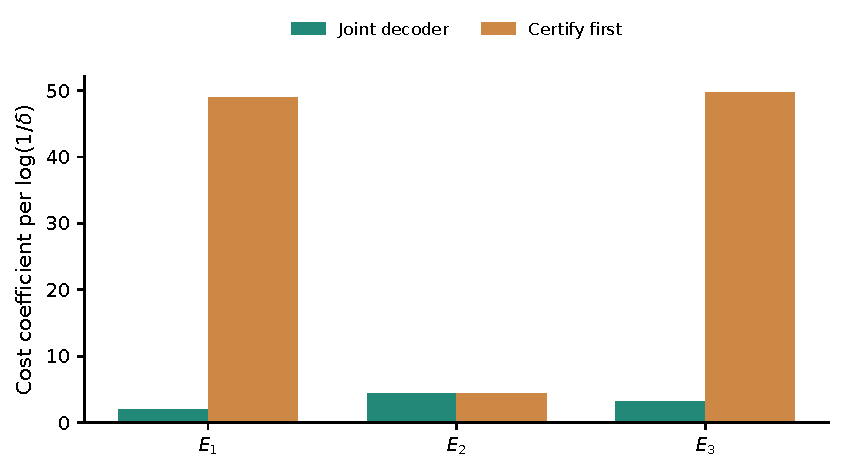
\includegraphics[width=.82\linewidth]{figures/certification_coefficients.pdf}
\caption{Fixed-instance asymptotic coefficients in the three-environment
example. Bars compare policy classes under the same old-label contract.}
\label{fig:coefficients}
\end{figure}

\subsection{A finite-deadline boundary of free post information}
For \eqref{eq:shrinking-example}, we evaluate the proved lower bound
\eqref{eq:deadline-cost-lower} at
$L_\delta=2,4,8,16,32,64,128,256$, using $H=L_\delta^2$.
These curves are analytic lower-bound evaluations; no purported exact
large-horizon certification optimizer is run. In $E_1$ the normalized bound
approaches the separated coefficient $48.9931965$, as proved by
Theorem~\ref{thm:collapse}. Every frozen post experiment has a universal
decoder, but the varying family has this positive leading coefficient.

\begin{figure}[ht]
\centering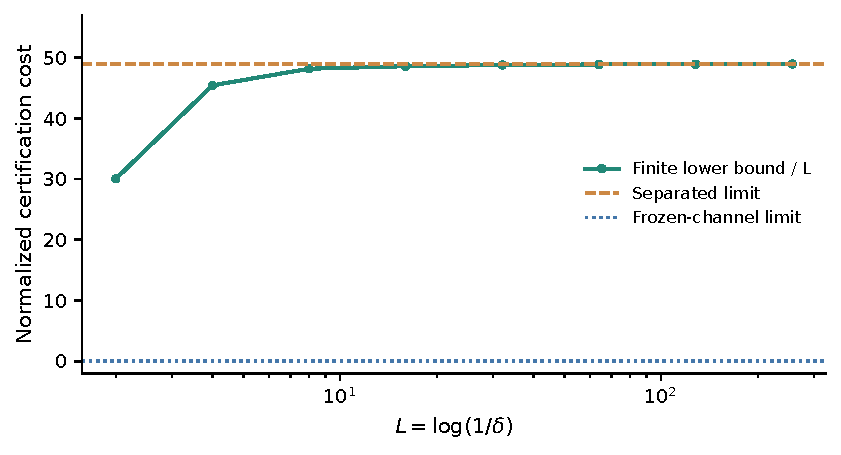
\includegraphics[width=.83\linewidth]{figures/shrinking_channel.pdf}
\caption{For $E_1$, finite information lower bound divided by $L_\delta$
along the shrinking-channel family, compared with its separated limit.
The zero line is the coefficient obtained when any one of the distinct post
experiments is frozen before sending the confidence level to zero.}
\label{fig:shrinking}
\end{figure}

\subsection{Current-label control in the original three-environment fixture}
This separate Bayes fixture has environments adequate, repairable, and
unrepairable, prior $(0.6,0.25,0.15)$, horizon $T=6$, and symmetric terminal
penalty $\lambda=0.5$. Old and new labels are $(1,0,0)$ and $(1,1,0)$;
their ordinary task costs are $(0,0.5,0.5)$ and $(0,0,0.5)$.
Every action takes one slot. In old mode, \KEEP{} has no information,
\VERIFY{} adds $0.08$ to the old task loss and yields Bernoulli means
$(0.2,0.8,0.8)$, and \REPAIR{} adds $0.2$ to old task loss and succeeds
with probability $0.8$ in every environment. Failure leaves the old mode
available for another attempt. The repair affects the \emph{next} task.
New-mode tasks yield Bernoulli means $(0.1,0.1,0.9)$.
Fallback costs $0.12$ per round, gives no information, and preserves whether
the installed representation is old or new. There are four visible modes.

The original gate restricts \REPAIR{} only, at posterior threshold $0.95$;
fallback remains available. This is neither the old-label commitment class
nor exactly the two-action gate definition used for the binary theorems.
Both its action set and its threshold are recorded in the model.
\begin{table}[ht]
\centering\small\begin{tabular}{lllrrr}
\toprule
Policy & Bayes cost & First action & $e_1$ & $e_2$ & $e_3$\\
\midrule
joint & 0.73146152 & repair & 0.036824 & 0.036824 & 0.017384\\
gate\_095 & 0.83414400 & verify & 0.232000 & 0.072000 & 0.072000\\
no\_repair & 0.83414400 & verify & 0.232000 & 0.072000 & 0.072000\\
\bottomrule
\end{tabular}

\caption{Exact current-label Bayes fixture, rounded for display.
The $e_i$ columns are conditional terminal errors under the same implemented
policy; no uniform $\delta$ constraint is imposed.}\label{tab:original-bayes}
\end{table}
The joint cost is exactly $9143269/12500000=0.73146152$; the two restricted
costs are $26067/31250=0.834144$. Initial actions are repair and verify,
respectively. Conditional errors agree with the independently reconstructed
original values.

A threshold sweep also yields $0.834144$ at threshold $0.5$ for this same
repair-only gate. Thus the default gap is not solely an artifact of imposing
$0.95$. The sweep evaluates explicit alternative restrictions and does not
turn a posterior gate into a frequentist confidence guarantee.

One-at-a-time sensitivity varies repair fee over $0,0.1,0.2,0.4,0.8$,
success probability over $0,0.2,0.5,0.8,1$, verification accuracy over
$0.5,0.65,0.8,0.95,1$, and horizon over $1,2,4,6,8$. All values and
first actions are in Appendix~\ref{app:original-sensitivity}.
The maximum difference from the supplied source archive's cost and error
columns is approximately $2.3\times10^{-13}$. Timeout residuals are treated
separately as described above.

\begin{figure}[ht]
\centering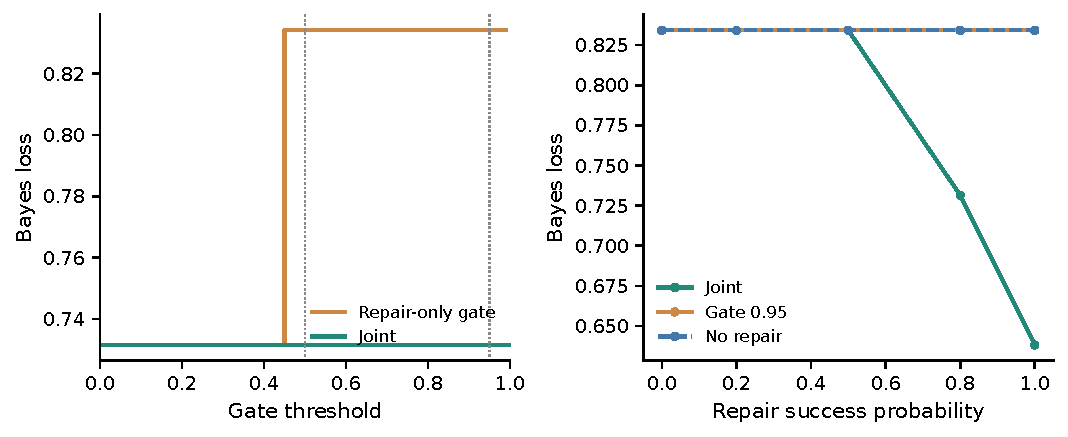
\includegraphics[width=.95\linewidth]{figures/original_sensitivity.pdf}
\caption{Current-label fixture. Left: repair-only gate as its threshold
varies, with unrestricted value as a reference. Right: values as repair success
varies at the original $0.95$ gate. Policies share all other primitives
within each comparison.}\label{fig:original-sensitivity}
\end{figure}

\subsection{Binary families and repair-region geometry}
Nine binary configurations retain the finite-horizon development:
F0 fixes the representation; F1 is the no-information benchmark;
F2 uses perfect verification; F3 uses full-support noisy verification;
F4 allows fallback and deferral; F5 has one repair attempt with success
probabilities $(3/4,1/2)$; F6 adds passive post information;
F7 is unidentifiable; and F8 is the exact one-round two-region example.
Complete rational parameters are stored in the configurations.
Unlike the three-environment fixture, these repairs affect the current task.
For F0--F7 verification retains old task loss in addition to its price.
For F8 and the repair-region sweep it replaces the round's ordinary task.
No comparison changes this convention between policies.

The joint and gate policies optimize their respective menus exactly.
Stage-myopic minimizes immediate cost; greedy-VOI minimizes immediate cost
plus the one-action terminal Bayes risk. Verify-then-act verifies once initially
and subsequently disables verification. Never-repair retains other actions;
always-repair forces the first repair and then optimizes. All use the same
optimal terminal declaration. The environment oracle knows the true index
only to provide a lower bound.
\begin{table}[ht]
\centering\small\begin{tabular}{lrrrrr}
\toprule
Instance & Oracle & Joint & Gate & Myopic & Gate gap\\
\midrule
F0 & 2.4000 & 3.0000 & 3.0000 & 3.0000 & 0.0000\\
F1 & 0.3000 & 4.8000 & 6.3000 & 6.3000 & 1.5000\\
F2 & 0.0300 & 1.1200 & 1.1300 & 1.1200 & 0.0100\\
F3 & 0.0300 & 1.4000 & 2.1300 & 1.4000 & 0.7300\\
F4 & 0.3000 & 2.6400 & 2.6400 & 3.6000 & 0.0000\\
F5 & 0.7200 & 2.3075 & 2.6520 & 2.3700 & 0.3445\\
F6 & 0.0300 & 0.9466 & 1.9290 & 0.9466 & 0.9825\\
F7 & 0.7800 & 1.9750 & 3.6000 & 1.9750 & 1.6250\\
F8 & 0.0250 & 0.7500 & 0.9000 & 0.7500 & 0.1500\\
\bottomrule
\end{tabular}

\caption{Binary Bayes benchmarks. Exact fractions and all seven policy
columns are provided in the CSV. A positive gate gap is not universal.}
\label{tab:benchmark}
\end{table}
F1 gives the exact gap $3/2$ and F8 the noisy gap $3/20$.
F4 has equal joint and gate values. Comparing F3 with F6, passive information
reduces joint loss from $1.4$ to $0.94656$ and gate loss from $2.13$ to
$1.92904$, while their gap increases. Better information therefore need not
reduce the difference between these two policy classes.

\begin{figure}[ht]
\centering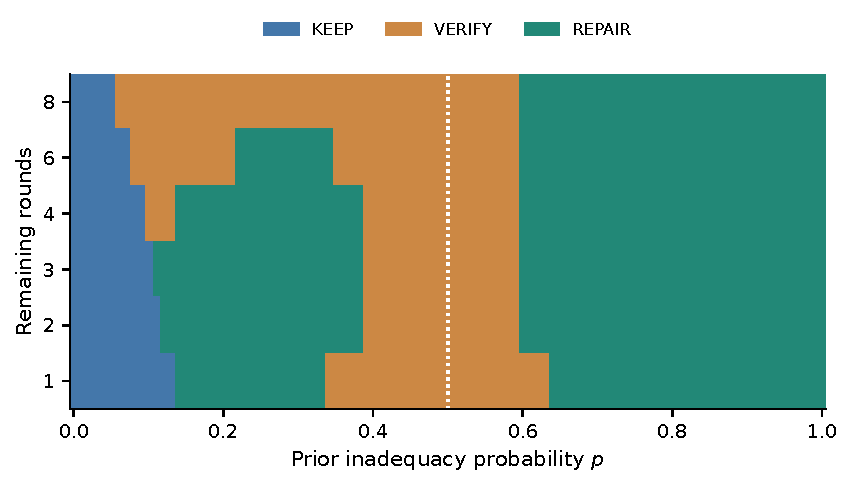
\includegraphics[width=.88\linewidth]{figures/horizon_regions.pdf}
\caption{Exact actions on 101 rational priors at six horizons.
Interpolation between sampled priors is illustrative; only the one-round
boundaries in Theorem~\ref{thm:counter} have the stated analytic endpoints.}
\label{fig:regions}
\end{figure}
\begin{figure}[ht]
\centering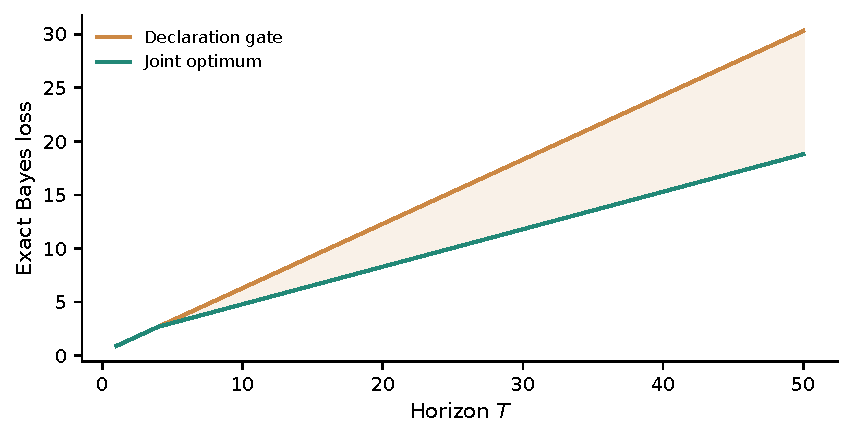
\includegraphics[width=.84\linewidth]{figures/no_information_gap.pdf}
\caption{The exact no-information gap is $\max(0,T/4-1)$ at the F1 parameters.
All displayed values agree with the rational solver.}\label{fig:noinfo}
\end{figure}
\begin{figure}[ht]
\centering
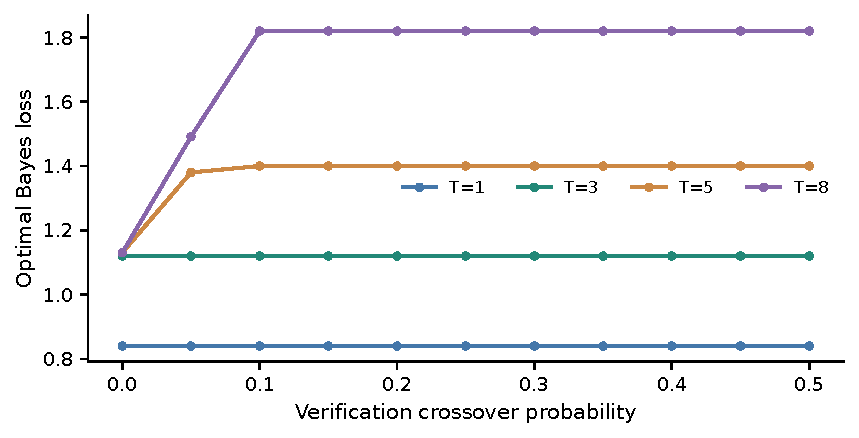
\includegraphics[width=.82\linewidth]{figures/blackwell.pdf}\\[5pt]
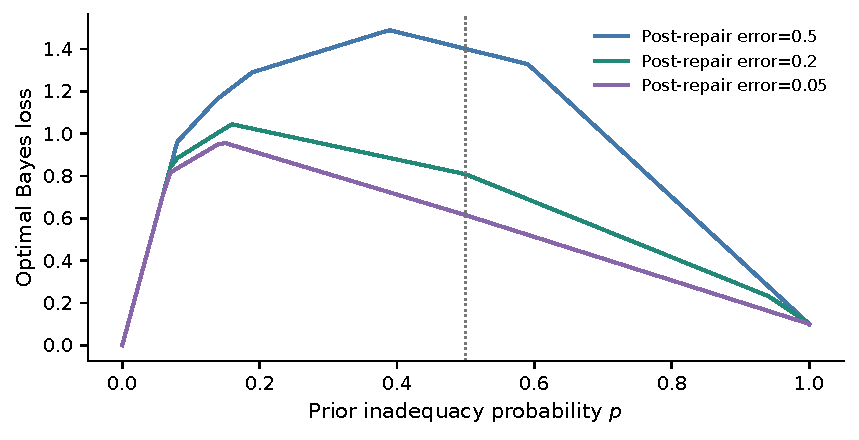
\includegraphics[width=.82\linewidth]{figures/post_information.pdf}
\caption{Top: unrestricted value under a pure verification channel comparison
at fixed costs. Bottom: values for three passive post-repair channels.
These are finite value calculations, not general monotonicity claims for
the gate gap.}\label{fig:information}
\end{figure}

The long-horizon fixed-prefix illustration in Figure~\ref{fig:log}
tests $0\le n\le\min(100,T-1)$. At $T=1000$ it selects $n=15$ and
has loss approximately $17.02328$. Subtracting the oracle $0.3$ gives
a valid gate-gap upper bound $16.72328$, not the optimal gated value.

\subsection{Independent checks and computational limits}
The policy-tree enumerator never updates a posterior or invokes the Bellman
solver. It enumerates environment-wise loss vectors for all deterministic
trees, retaining duplicates, and then minimizes their prior inner products.
All 20 binary prior--horizon comparisons and all 12 three-environment
comparisons have exactly zero rational difference. The largest enumerated
tree family has 61,872 policies.

The 32-test suite checks exact thresholds and endpoints, factorized versus
enumerated decoder coefficients and eligibility, equality-at-threshold ties,
global decoder tie breaking, the two finite protocol implementations,
visible success information, aggregation, multi-slot action completion,
fallback labels, asymmetric errors, abstention, serialization, gate menus,
and a $10^{-12}$-probability branch with $10^{12}$ loss. Tests of the new
structural formulas supplement their proofs; they do not establish
mathematical priority or formal verification.

For $N_b$ cached belief nodes, at most $A$ actions and $O$ joint observable
outcomes, Bellman computation uses $O(N_bAOK)$ rational operations, excluding
integer bit complexity. The number of nodes can grow exponentially in the
horizon. The supplied binary timing family grows from five cached nodes at
one round to 313 at twelve rounds; this is an instance-specific count.
An online factorized decoder check is polynomial in $K$, but a Bernoulli
count-lattice evaluator handles $O(N^2)$ histories, each with its own
eligibility and post-tail calculation. These are separate complexity claims.
